\documentclass[11pt]{article}
\usepackage[margin=1in]{geometry}
\usepackage{amsmath,amssymb}
\usepackage{graphicx}
\usepackage{booktabs}
\usepackage{pgfplots}
\pgfplotsset{compat=1.18}
\usepackage[numbers,sort&compress]{natbib}
\usepackage[hidelinks]{hyperref}
\usepackage{microtype}
\usepackage{caption}
\captionsetup{font=small}

\title{What Does a Neural Simulation Tick Cost?\\
\large A Cost-Normalized Evaluation of a Sparse GPU Simulator}
\author{zxcAsD01\\
\small Independent researcher\\
\small \url{https://github.com/zxcAsD01-d/Neurosim-GPU}}
\date{October 2026}

\begin{document}
\maketitle

\begin{abstract}
Neural simulators are usually evaluated against other simulators, which mixes
algorithmic differences with implementation quality. We argue for a narrower and
more portable denominator: the cost of one sparse matrix multiplication over the
same synapses, on the same device, with the same batch. We present a
fixed-topology sparse simulator built around that accounting and report what the
denominator reveals. On a laptop GPU, a complete neural tick---sparse reduction,
$\tanh$, leak, gain and clip---costs $0.74$--$0.82\times$ a same-parameter
\texttt{cuSPARSE} multiplication at batch one and $2.8$--$6.6\%$ more than a
matching custom SpMM; the fused kernel beats the library call only because it
fuses work the library cannot. Persistent-current event propagation is
$3.0$--$4.5\times$ faster than the matrix path when $2.6\%$ of edges emit, and on
trained MNIST networks propagating one fifth of the edges changes accuracy by
$0.1$ percentage points. We also report where the approach does \emph{not} pay:
the reference event path is $5$--$81\times$ slower than dense propagation on CPU,
eligibility scanning destroys whole-tick event sparsity, and a dopamine-gated
online plasticity rule produced no measurable behavioural change in our control
task---an ablation shows the rule had no leverage on the synapses that mattered.
We release the implementation, 105 experiment runs, raw payloads and a
device-agnostic performance harness so that every number can be regenerated or
contradicted.
\end{abstract}

\section{Introduction}

Simulation papers usually answer ``how fast is your simulator?'' by comparing
against another simulator. That comparison is useful, but it confounds three
different things: the cost of the sparse linear algebra the model requires, the
cost of the neural update around it, and the engineering quality of the
implementation. A simulator can win the comparison by being faster at sparse
math, or lose it for reasons that have nothing to do with the model.

This paper takes the position that a neural simulator should first be measured
against \emph{the sparse operation it is made of}. For a fixed topology with $M$
synapses, $N$ neurons and batch $B$, one tick is
\begin{align}
  c_t &= W\,s_t + d_t, \\
  s_{t+1} &= \operatorname{clamp}\!\big(\alpha \odot s_t + (1-\alpha)\odot g\odot
             \tanh(c_t),\,0,\,1\big),
\end{align}
with $W$ sparse, $s_t\in[0,1]^{B\times N}$, and per-neuron leak $\alpha$ and gain
$g$. The work is $O(BM + BN)$. The interesting question is not whether this is
asymptotically a sparse matrix multiplication---it is---but how much the
\texttt{tanh}, the leak, the clip, the Python dispatch and the memory traffic add
on top of it in practice.

We built a simulator around this question and report four kinds of evidence.
First, \emph{tick parity}: the fused tick against a same-parameter sparse
multiplication on the same device. Second, \emph{event parity}: what happens when
only state deltas above a threshold are propagated, both in time and in accuracy
on trained networks. Third, \emph{task evidence} on MNIST digits and an inverted
pendulum, including negative results. Fourth, a \emph{reproducibility artifact}:
the implementation, the experiment grid, the raw payloads and the scripts that
regenerate the tables in this paper.

\paragraph{Contributions.}
\begin{enumerate}
  \item A cost-normalized evaluation protocol for sparse neural simulation that
        separates simulator overhead from sparse-math cost, with two
        denominators (a library SpMM and a matching custom SpMM) and explicit
        controls (same topology, weights, batch, activity, and device state).
  \item Measurements of a fused sparse tick from $1$M to $50$M synapses:
        $0.74$--$0.82\times$ the \texttt{cuSPARSE} denominator at batch one,
        $1.15\times$ at batch eight, and $2.8$--$6.6\%$ over a matching custom
        SpMM.
  \item A bounded-error characterization of emitted-event propagation on
        \emph{trained} weights rather than random ones: propagating $21\%$ of
        edges costs $0.11$ accuracy points on MNIST, $8.4\%$ costs $0.55$.
  \item A negative result with a diagnostic: dopamine-gated three-factor
        plasticity produced no behavioural change in a closed-loop control task,
        and an ablation shows why---zeroing every recurrent weight still left
        $193.8/200$ survival steps, so the rule had no leverage.
  \item An explicit account of where event sparsity stops paying: eligibility
        scanning is $O(BM)$ per tick, and the reference event scatter is slower
        than dense propagation on CPU.
\end{enumerate}

We do not claim a new simulation algorithm. Sparse spiking simulation,
event-driven propagation and three-factor plasticity are mature ideas; the
contribution is measurement discipline, an integrated reference implementation,
and a clear statement of what the numbers do and do not support.

\section{Related Work}

Brian~2 provides a mature, equation-oriented simulator with strong CPU and
code-generation performance \citep{stimberg2019brian2}; NEST targets
large-scale distributed networks \citep{gewaltig2007nest}; GeNN generates
device code for GPU execution \citep{yavuz2016genn}. Reviews of the design space
date back to \citet{brette2007simulation}. Event-driven simulation of networks
with delays and dynamic synapses has a long history
\citep{mattia2000efficient}, and the practical question of when it beats
time-driven simulation is exactly the trade-off we quantify here.

On the learning side, three-factor plasticity rules that combine a local
eligibility trace with a neuromodulatory signal are well established
\citep{fremaux2016neuromodulated}, and the dopamine reward-prediction-error
interpretation is standard \citep{schultz1997neural}. Libraries such as Norse
\citep{pehle2021norse} and snnTorch \citep{eshraghian2023training} make spiking
layers usable inside autodiff frameworks, while neuromorphic hardware such as
Loihi explores on-chip learning \citep{davies2018loihi}. Our implementation uses
PyTorch \citep{paszke2019pytorch} for the reference paths and a small custom CUDA
extension for the fused paths.

Relative to this literature, our claim is deliberately modest: we do not propose
a better simulator, but a way to report what a simulator costs, and a set of
measurements that other implementations can be compared against.

\section{System}

\subsection{State and topology}

The topology is a fixed directed multigraph with $N$ neurons and $M$ synapses
after coalescing duplicate edges. Two views are materialized: a canonical
source-major edge list (source, destination, weight) used by event propagation,
and a destination-major CSR view used by the matrix path. A monotonic
\emph{weight version} lets a persistent-current runtime detect out-of-band weight
changes and rebuild its cached current. Positions, chemical concentrations,
eligibility and delay history each have a single owner and a documented lifetime;
the ownership table is part of the repository documentation.

\subsection{Runtimes}

Four paths share the same state layout:
\begin{itemize}
  \item \textbf{Matrix} (reference): one \texttt{torch.sparse.mm} per tick plus
        elementwise update.
  \item \textbf{Persistent current (PELS)}: keeps $W s^{\text{emit}}$ as state
        and propagates only emitted deltas; mathematically equivalent to the
        matrix path at threshold zero.
  \item \textbf{Native matrix}: one fused CUDA kernel over a single
        destination-major weight array.
  \item \textbf{Native event}: fused advance, compaction and source-major
        scatter.
\end{itemize}
The first two are portable and readable; the last two are the performance paths
and are inference-only. Training uses the matrix path or a pointwise native
adjoint, never the event kernel.

\subsection{Emitted-event propagation}

Each tick produces a state delta $\Delta s = s_{t+1} - s^{\text{emit}}$. Edges
whose source delta is below a threshold $\theta$ are not traversed; instead the
persistent current is updated by scattering only the retained deltas:
\begin{equation}
  c \leftarrow c + W\,\mathbf{1}[|\Delta s| \ge \theta] \odot \Delta s .
\end{equation}
With $\theta = 0$ this is the matrix path. With $\theta > 0$ the error is bounded
per tick by the suppressed delta mass, but it compounds across ticks; the
repository treats the threshold as a contract parameter with a validation
protocol, not as a free knob.

\subsection{Neurochemistry and schedule}

A regional dopamine field supports tonic, burst and dip components, volume-weighted
diffusion, uptake, transport delay, autoreceptor feedback and D1/D2 Hill
occupancy. Plasticity is three-factor: pre/post traces form a per-edge
eligibility, and a dopamine signal gates a sign-preserving weight update. These
run at their own cadence---chemistry every $K_c$ ticks, migration every $K_m$,
structural change every $K_s$---so the neural tick stays $O(BM + BN)$ while the
slow processes pay their cost only when they run.

\section{Cost-Normalized Evaluation}

\subsection{Denominators}

We report two ratios. The \emph{library ratio} is
$\rho_{\text{lib}} = T_{\text{tick}} / T_{\text{cuSPARSE}}$, where the
denominator is a sparse multiplication with the same $W$, batch and dtype,
measured on the same device in the same session. The \emph{matching ratio} is
$\rho_{\text{match}} = T_{\text{tick}} / T_{\text{SpMM}}$, where the denominator
is our own destination-major SpMM kernel without the elementwise update.

The two answer different questions. $\rho_{\text{lib}}$ is what a user gets by
replacing a library call with the simulator; it can be below one because fusion
removes intermediate traffic. $\rho_{\text{match}}$ isolates the cost of the
neural update itself. Reporting only one of them invites the wrong conclusion:
$\rho_{\text{lib}} < 1$ does not mean the dynamics are free, and
$\rho_{\text{match}} \approx 1$ does not mean a library swap is a win.

\subsection{Metrics and controls}

We report per-tick time (median after warmup), full-graph-equivalent throughput
in synapses per second, bytes per synapse for the deployed layouts, and, for the
event path, the fraction of edges that actually emit. Controls: identical
topology object and weights across runtimes; identical initial state and drive;
batch and dtype fixed; the device otherwise idle; topology construction and JIT
compilation outside the timed region.

For accuracy claims we use a different harness entirely (Section~\ref{sec:tasks}),
because a fast tick that computes the wrong thing is not a result.

\section{Results}

\begin{figure}[t]
\centering
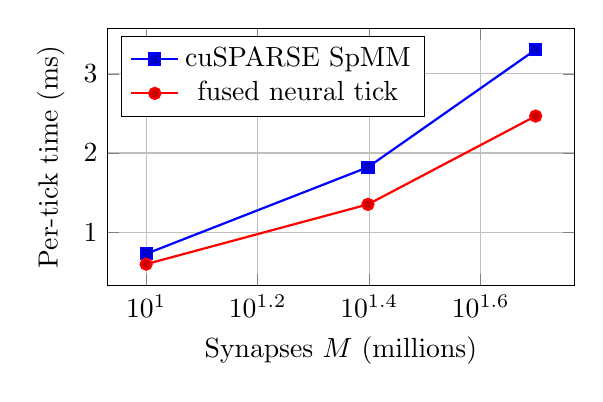
\begin{tikzpicture}
\begin{axis}[width=0.62\textwidth, height=0.4\textwidth, xlabel={Synapses $M$ (millions)}, ylabel={Per-tick time (ms)}, grid=both, xmode=log, legend pos=north west]
\addplot+[mark=square*, thick] coordinates {(10.00,0.725) (24.99,1.820) (49.95,3.305)};
\addplot+[mark=*, thick] coordinates {(10.00,0.595) (24.99,1.350) (49.95,2.466)};
\legend{cuSPARSE SpMM, fused neural tick}
\end{axis}
\end{tikzpicture}
\caption{Fixed-topology tick cost against a same-parameter cuSPARSE multiplication (RTX 5070 Laptop, batch 1). The complete neural update is cheaper than the library denominator because it fuses the elementwise work.}
\label{fig:tick}
\end{figure}


\subsection{Tick parity}

Table~\ref{tab:gpu-core} and Figure~\ref{fig:tick} summarize the GPU
measurements (RTX 5070 Laptop, 8\,GiB, CUDA 13.1, FP32). At batch one the
complete tick costs $0.821\times$, $0.742\times$ and $0.746\times$ the
\texttt{cuSPARSE} denominator at $10$M, $25$M and $50$M synapses. Against the
matching custom SpMM the same ticks cost $1.066\times$, $1.028\times$ and
$0.918\times$: the neural update adds $2.8$--$6.6\%$ over the sparse reduction,
and at the largest graph the fused kernel is slightly cheaper than the matching
SpMM alone because the state update is folded into the reduction pass.

\begin{table}[t]
\centering
\small
\caption{GPU tick parity. ``raw'' is a same-parameter \texttt{cuSPARSE}
multiplication, ``canonical'' our destination-major SpMM without the update,
``fused'' the complete tick. Batch one except the last row.}
\label{tab:gpu-core}
\begin{tabular}{rrrrrrr}
\toprule
$N$ & $M$ & $B$ & raw (ms) & canonical (ms) & fused (ms) & fused/raw \\
\midrule
166k & 10.00M & 1 & 0.725 & 0.558 & 0.595 & 0.821 \\
166k & 24.99M & 1 & 1.820 & 1.313 & 1.350 & 0.742 \\
166k & 49.95M & 1 & 3.305 & 2.686 & 2.466 & 0.746 \\
50k  & 1.00M  & 8 & 0.447 & 0.460 & 0.513 & 1.148 \\
\bottomrule
\end{tabular}
\end{table}

At batch eight the picture changes: $1.148\times$ the library denominator and
$1.115\times$ the matching SpMM. The elementwise work now has more data per
synapse to move, and the fused kernel loses the batch-one advantage. This is the
expected shape---fusion helps when the arithmetic intensity is low---but it is
worth stating because it bounds the claim: the parity result is a batch-one
result.

\subsection{Event sparsity}

With $\theta = 0.05$ and $20$ warmup ticks, $2.64\%$ of edges emit. The native
event kernel then takes $0.200$\,ms versus $0.595$\,ms for the matrix tick at
$10$M synapses, $0.301$ versus $1.350$\,ms at $25$M, and $0.123$ versus
$0.513$\,ms at $1$M with batch eight: a $3.0$--$4.5\times$ speedup.

The more interesting question is what this costs in accuracy. We trained $56$
sparse-brain configurations on MNIST (varying width, degree, ticks, data and
leak), then re-ran each through the persistent-current runtime at several
thresholds. Table~\ref{tab:theta} and Figure~\ref{fig:theta} aggregate the
result: $37.6\%$ of edges active at $\theta = 0.05$ changes accuracy by
$+0.01$ percentage points, $21.3\%$ active at $\theta = 0.1$ costs $0.11$ points,
and $8.4\%$ active at $\theta = 0.2$ costs $0.55$ points.

\begin{table}[t]
\centering
\small
\caption{Emitted-event threshold on MNIST, aggregated over 53 trained sparse-brain configurations. Accuracy is measured through the persistent-current runtime, so $\theta>0$ is the bounded-error path; $\Delta$ is relative to the same run's matrix-path accuracy.}
\label{tab:theta}
\begin{tabular}{rrrr}
\toprule
$\theta$ & Accuracy (\%) & $\Delta$ (pp) & Active edges (\%) \\
\midrule
0.00 & 90.29\,$\pm$\,2.79 & +0.00 & 96.2 \\
0.02 & 90.29\,$\pm$\,2.84 & -0.00 & 59.9 \\
0.05 & 90.30\,$\pm$\,2.72 & +0.01 & 37.6 \\
0.10 & 90.18\,$\pm$\,2.75 & -0.11 & 21.3 \\
0.20 & 89.74\,$\pm$\,2.55 & -0.55 & 8.4 \\
\bottomrule
\end{tabular}
\end{table}

\begin{figure}[t]
\centering
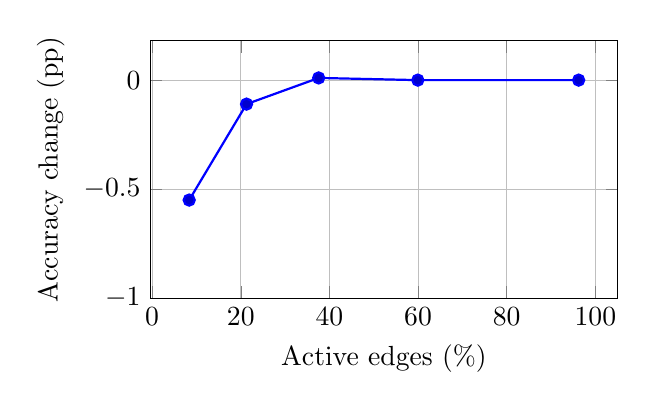
\begin{tikzpicture}
\begin{axis}[width=0.62\textwidth, height=0.4\textwidth, xlabel={Active edges (\%)}, ylabel={Accuracy change (pp)}, grid=both, ymin=-1.0, ymax=0.18]
\addplot+[mark=*, thick] coordinates {(96.23,0.00) (59.94,-0.00) (37.57,0.01) (21.30,-0.11) (8.36,-0.55)};
\end{axis}
\end{tikzpicture}
\caption{Bounded-error event propagation: accuracy change against the fraction of edges that emit, averaged over 56 trained sparse-brain configurations. Propagating one fifth of the edges costs about a tenth of a point.}
\label{fig:theta}
\end{figure}


Two caveats matter. First, this measures forward propagation only. With
eligibility enabled, the dopamine runtime still scans all $M$ edges per tick, so
whole-tick event sparsity requires eligibility to be off and no weight update to
occur on that tick. Second, the activity fraction depends on the dynamics and the
warmup, not on $\theta$ alone: the same threshold produced $2.64\%$ activity in
the GPU benchmark and tens of percent on the MNIST runs. The relationship between
active edges and accuracy is the transferable result, not the threshold value.

\subsection{Memory}

The mutable topology stores two endpoints, two weight views, two row-pointer
arrays and a permutation: $24M + 8N$ bytes, or $3.0$\,GB at $125$M synapses. A
read-only inference view uses one weight array plus event indices, about
$16M + 8N$ bytes, or $2.0$\,GB. Measured bytes per synapse range from $24.2$ to
$25.0$ for $N$ between 2k and 32k, consistent with the layout. These constants are
structural, not implementation accidents: removing a view or an index array
changes the constant, not the scaling.

\subsection{Training}

Forward and backward for a same-parameter sparse RNN ($N = 16{,}384$,
$M = 998{,}187$, $B = 4$, $T = 32$) take $185.6$\,ms. PyTorch matrix dynamics
take $209.9$\,ms ($1.131\times$); the native fused pointwise dynamics take
$199.5$\,ms ($1.075\times$, $93\%$ same-parameter efficiency). The native
analytic pointwise backward removes about half of the overhead ($13.1\% \to
7.5\%$). Sparse-weight backward still uses \texttt{cuSPARSE}; a fused
whole-rollout adjoint is not implemented, and we do not claim training is free:
$7.5\%$ is a cost, not a speedup.

\subsection{Task evidence}
\label{sec:tasks}

All task experiments run on CPU, in pure PyTorch, and are \emph{not} performance
measurements; they exist to check that the stack learns and controls, and to
expose failure modes. Table~\ref{tab:models} and Figure~\ref{fig:params} report
MNIST accuracy at $10$k training digits, $10$ epochs, three seeds.

\begin{table}[t]
\centering
\small
\caption{MNIST test accuracy (10{,}000 training samples, 10 epochs, 3 seeds; mean $\pm$ population standard deviation). ``Params'' counts trainable scalars; ``synapses'' counts coalesced edges of the fixed topology.}
\label{tab:models}
\begin{tabular}{lrrr}
\toprule
Model & Test accuracy (\%) & Params & Synapses \\
\midrule
Logistic regression & 91.8\,$\pm$\,0.3 & 7,850 & -- \\
MLP, $h=6$ & 87.3\,$\pm$\,0.9 & 4,780 & -- \\
MLP, $h=64$ & 94.7\,$\pm$\,0.0 & 50,890 & -- \\
Sparse brain ($N{=}256$, $d{=}8$, $T{=}8$) & 91.1\,$\pm$\,0.2 & 4,586 & 2,016 \\
Dense RNN ($N{=}256$, $T{=}8$) & 95.0\,$\pm$\,0.3 & 269,066 & -- \\
\bottomrule
\end{tabular}
\end{table}

\begin{figure}[t]
\centering
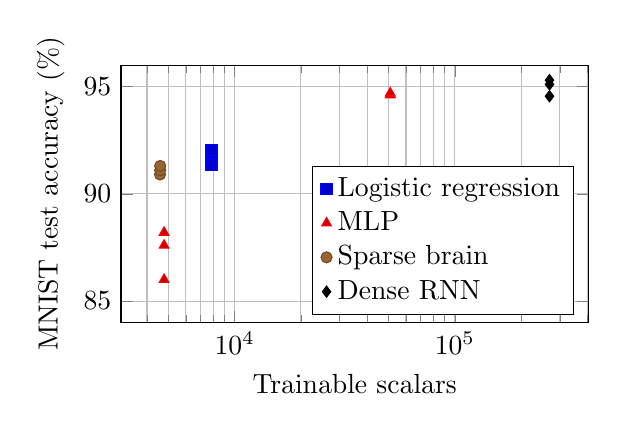
\begin{tikzpicture}
\begin{axis}[width=0.62\textwidth, height=0.4\textwidth, xlabel={Trainable scalars}, ylabel={MNIST test accuracy (\%)}, xmode=log, grid=both, legend pos=south east, legend cell align=left, ymin=84, ymax=96]
\addplot+[mark=square*, only marks] coordinates {(7850,91.35) (7850,91.90) (7850,92.05)};
\addplot+[mark=triangle*, only marks] coordinates {(4780,86.00) (4780,87.60) (4780,88.20) (50890,94.60) (50890,94.65) (50890,94.70)};
\addplot+[mark=*, only marks] coordinates {(4580,90.90) (4588,91.10) (4589,91.30)};
\addplot+[mark=diamond*, only marks] coordinates {(269066,94.55) (269066,95.10) (269066,95.30)};
\legend{Logistic regression, MLP, Sparse brain, Dense RNN}
\end{axis}
\end{tikzpicture}
\caption{Parameter efficiency on MNIST (10k training digits, 3 seeds). The sparse brain sits at 4.6k trainable scalars between the parameter-matched MLP and the wide baselines; it does not beat a linear classifier.}
\label{fig:params}
\end{figure}


A sparse brain with $4{,}586$ trainable scalars reaches $91.1\%$, against
$87.3\%$ for a parameter-matched MLP ($4{,}780$ scalars) and $91.8\%$ for logistic
regression ($7{,}850$). The fixed sparse recurrence is worth $6.3$ points over the
same architecture without recurrence ($84.7\%$), so the gain is not merely a
random projection. But the absolute accuracy is below a linear classifier and far
below a wide MLP ($94.7\%$) or a dense RNN with $59\times$ the parameters
($95.0\%$). Fixed topology buys parameter efficiency, not accuracy.

Under additive Gaussian input noise (Figure~\ref{fig:noise}) the ordering
reverses. At $\sigma = 0.3$ the sparse brain reaches $72.9\%$, against $55.1\%$
for the wide MLP and $57.3\%$ for logistic regression; at $\sigma = 0.2$ the gap
is $84.4\%$ versus $74.8\%$. The saturating dynamics appear to act as a bounded
denoiser, while the ReLU baselines propagate noise to the readout. The advantage
does not extend to occlusion, where the sparse brain is slightly worse, or to a
two-pixel shift, where it is in the middle of the pack. Robustness is
direction-dependent.

\begin{figure}[t]
\centering
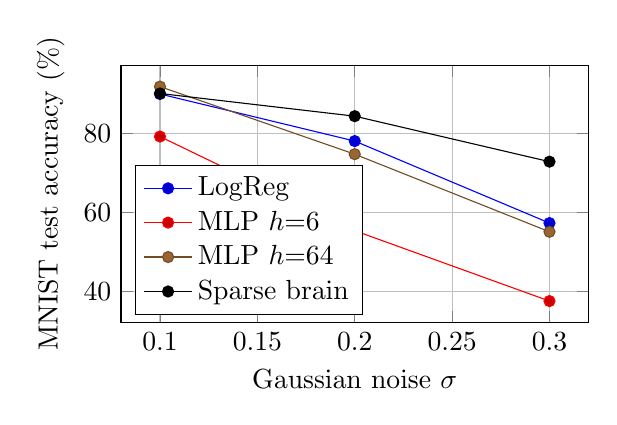
\begin{tikzpicture}
\begin{axis}[width=0.62\textwidth, height=0.4\textwidth, xlabel={Gaussian noise $\sigma$}, ylabel={MNIST test accuracy (\%)}, grid=both, legend pos=south west, legend cell align=left]
\addplot+[mark=*] coordinates {(0.10,90.05) (0.20,78.10) (0.30,57.28)};
\addplot+[mark=*] coordinates {(0.10,79.25) (0.20,55.35) (0.30,37.48)};
\addplot+[mark=*] coordinates {(0.10,91.93) (0.20,74.77) (0.30,55.07)};
\addplot+[mark=*] coordinates {(0.10,90.18) (0.20,84.42) (0.30,72.87)};
\legend{LogReg, MLP $h{=}6$, MLP $h{=}64$, Sparse brain}
\end{axis}
\end{tikzpicture}
\caption{Accuracy under additive Gaussian input noise (3 seeds). The saturating sparse core degrades more slowly than the ReLU baselines at high noise.}
\label{fig:noise}
\end{figure}


On the inverted pendulum (Table~\ref{tab:cartpole}) both cloned policies sit at
the $200$-step ceiling, so imitation accuracy ($96.7\%$ versus $88.7\%$) does not
translate into a closed-loop difference. Failures require extreme conditions
(Table~\ref{tab:robustness}): action delay of six steps collapses both policies
to about $30$ steps, and noise $\sigma = 0.2$ degrades both. The failure
direction differs---the sparse brain loses stability under delay four while the
MLP remains at ceiling, and a four-fold pole length collapses the MLP
($38.8$ steps) while the sparse brain survives ($198.7$)---which suggests
different frequency responses rather than a general robustness ranking.

\begin{table}[t]
\centering
\small
\caption{Cart-pole closed-loop evaluation (100 episodes, 3 seeds). Survival is out of 200 steps; success requires $\geq 195$ steps. Angle RMS is in degrees. BC accuracy is the held-out imitation accuracy.}
\label{tab:cartpole}
\begin{tabular}{llrrrr}
\toprule
Policy & Protocol & Survival & Success (\%) & Angle RMS & BC (\%) \\
\midrule
LQR & nominal & 200.0 & 100 & 0.36 & -- \\
MLP (BC) & nominal & 200.0 & 100 & 0.36 & 96.7 \\
Sparse brain (BC) & nominal & 200.0 & 100 & 0.36 & 88.7 \\
LQR & hard & 200.0 & 100 & 0.96 & -- \\
MLP (BC) & hard & 200.0 & 100 & 0.97 & 96.2 \\
Sparse brain (BC) & hard & 200.0 & 100 & 1.12 & 85.0 \\
\bottomrule
\end{tabular}
\end{table}

\begin{table}[t]
\centering
\small
\caption{Robustness grid on the hard protocol (40 episodes per condition, 2 seeds): mean survival steps out of 200. Both policies sit at the ceiling for most conditions; the failures are informative.}
\label{tab:robustness}
\begin{tabular}{lrr}
\toprule
Condition & Sparse brain & MLP \\
\midrule
nominal & 200.0 & 200.0 \\
impulse & 200.0 & 200.0 \\
noise=0.1 & 197.3 & 200.0 \\
noise=0.2 & 102.2 & 127.9 \\
delay=1 & 200.0 & 200.0 \\
delay=2 & 200.0 & 200.0 \\
delay=4 & 162.8 & 200.0 \\
delay=6 & 37.2 & 29.1 \\
length\_scale=0.5 & 200.0 & 200.0 \\
length\_scale=2 & 193.7 & 200.0 \\
length\_scale=4 & 198.7 & 38.8 \\
mass\_scale=0.3 & 200.0 & 200.0 \\
mass\_scale=3 & 200.0 & 200.0 \\
\bottomrule
\end{tabular}
\end{table}


\subsection{A negative result, and why}

We tested whether dopamine-gated three-factor plasticity could adapt a cloned
policy after an unannounced plant change (actuator authority reduced from $6$\,N
to $1$\,N at episode ten). Frozen and online variants were statistically
indistinguishable: post-change survival $130.3$ versus $129.1$ steps over three
seeds, with online slightly worse. The rule did move weights ($\|\Delta W\| =
0.80$, about $8\%$ of the initial norm).

The ablation explains it. Zeroing every recurrent weight while keeping the
sensory projection and readout leaves $193.8/200$ survival steps on the hard
nominal protocol (seeds: $200.0$, $196.4$, $184.9$). The learned recurrence
contributes almost nothing to behaviour; the policy is driven by the fixed
feedforward path, so a rule that updates only recurrent weights has no lever.
This is not evidence against the plasticity rule. It is evidence that the
testbed, not the rule, was the limiting factor---and a reminder to run an
ablation before claiming that an online rule ``works''.

\subsection{The CPU reference path}

The portable matrix runtime is also measured on CPU (16 threads, PyTorch
2.14.0+cpu, median of 30 ticks). The complete tick costs $1.18$--$1.82\times$ a
raw sparse multiplication at batch one and $1.82$--$3.02\times$ at batch eight,
with throughput from $0.15$ to $2.9$ G synapses/s. The Python event scatter, by
contrast, is $5$--$81\times$ \emph{slower} than dense propagation. This is the
sharpest boundary in the paper: event sparsity is a property of the fused kernel.
A reference implementation that validates bounded error is not a performance
path, and reporting it as one would be wrong.

\section{Threats to Validity}

\paragraph{One device.} The GPU numbers come from one laptop
GPU and one driver/toolkit combination. We report the stack with every number,
and the harness is device-agnostic, but we have not reproduced them elsewhere.

\paragraph{No head-to-head comparison.} We compare against sparse primitives,
not against Brian~2, NEST, GeNN or Norse. A simulator-level comparison is the
natural next experiment and is not claimed here.

\paragraph{Scale.} The largest executed graph is $49.95$M synapses. The $125$M
point is a projection from measured throughput, not a measurement; the reason is
that random topology construction has a much larger temporary memory peak than
loading a prebuilt graph.

\paragraph{Activity depends on the run.} The event-path speedup is reported at
$2.64\%$ active edges, and the accuracy tables at $8$--$96\%$ depending on
$\theta$ and dynamics. Neither transfers to a different activity regime without
re-measurement.

\paragraph{Biology.} The neurochemical model is a functional proxy. Parameters
are not calibrated to recordings, and no biological claim is made.

\paragraph{Task probes.} Behaviour cloning is not reinforcement learning; the
ceiling is the LQR expert. The MNIST runs use $10$k training digits and three
seeds without significance testing, so relative ordering, not absolute
percentages, is the finding.

\section{Reproducibility}

The repository contains the implementation, the $105$-run experiment grid, the
raw JSON payloads, the aggregate tables and two harnesses: a device-agnostic
performance suite and a task-level suite. Accuracy and survival metrics are
seed-deterministic; latency is not. A CPU reference baseline is committed with
its machine profile. Every table in this paper is generated by
\texttt{paper/make\_assets.py} from the committed results, so a disagreement can
be traced to a payload rather than to prose. Documentation separates the source
of record for measurements from the interpretation and from the acceptance
criteria.

\section{Conclusion}

A sparse neural simulator should be able to say what one tick costs relative to
the sparse multiplication it is built on. On our measurements that ratio is
$0.74$--$0.82\times$ a library SpMM at batch one and $2.8$--$6.6\%$ over a
matching custom SpMM: the neural update is cheap, and the remaining cost is
memory movement and dispatch. Event propagation buys $3.0$--$4.5\times$ at low
activity and, on trained networks, costs about a tenth of an accuracy point at
one fifth of the edges. The approach stops paying when eligibility scanning or a
reference (non-fused) event path enters the picture, and an online plasticity
rule with no leverage on behaviour is indistinguishable from no rule at all.
Those boundaries are the useful part of the result.

\bibliographystyle{plainnat}
\bibliography{references}

\end{document}
